\section{Path-View: Neural Path Features and Information Flow}\label{sec:pathgate}
\textbf{Notation:} We consider fully connected deep networks with $d$ layers, and $w$ hidden units per layer, which accepts an input $x\in\R^{d_{in}}$, and produces an output $\hat{y}_{\Theta}\in \R$ where $\Theta\in\R^{d_{net}}$ ($d_{net}=w^2(d-2)+w(d_{in}+1)$). We denote by $\Theta(l,i,j)$ the weight connecting the $i^{th}$ hidden unit of layer $l-1$ to the $j^{th}$ hidden unit of layer $l$, and we use $G_{x,\Theta}(l,i)$ be the gating value ($0/1$) of the $i^{th}$ hidden unit in layer $l$ for an input $x\in \R^{d_{in}}$.\\
\textbf{Paths:}  We have a total of $P=d_{in}w^{(d-1)}$ paths. Let us say that an enumeration of the paths is given by $[P]=\{1,\ldots,P\}$. Let $\I_{l}\colon [P]\ra [w],l=0,\ldots,d-1$ provide the index of the hidden unit through which a path $p$ passes in layer $l$ (with the convention that $\I_d(p)=1,\forall p\in [P]$). The activity of a path $p$ for an input $x\in \R^{d_{in}}$ by $A_{\Theta}(x,p)\stackrel{def}{=}\Pi_{l=1}^{d-1} G_{x,\Theta}(l,\I_l(p))$.\\
\textbf{Gating:} In what follows, we consider two kinds of gates namely, i) hard gates, taking values in $\{0,1\}$, and ii) soft gates, taking values in $(0,1)$. For a pre-activation input $q\in\R$, the  hard and soft gates are given by $G_{R}(q)=\mathbbm{1}_{\{\q>0\}}$ and $G_{SR}(q)=\frac{1}{1+\exp(-\beta q)}$, where $\beta>0$ is a positive constant. Using the hard and soft gates, we can specify the ReLU and `soft-ReLU' activations as $\chi_{R}(q)=q\cdot\mathbbm{1}_{\{q>0\}}$ and $\chi_{SR}(q)=q\cdot\left(\frac{1}{1+\exp(-\beta q)}\right)$. Here, in $G$ and $\chi$, the subscripts $R$ and $SR$ stand for `ReLU' and `soft-ReLU' respectively.\\
\begin{figure*}[t]
%\begin{minipage}{0.78\columnwidth}
\resizebox{\columnwidth}{!}{
\begin{tabular}{ccc}
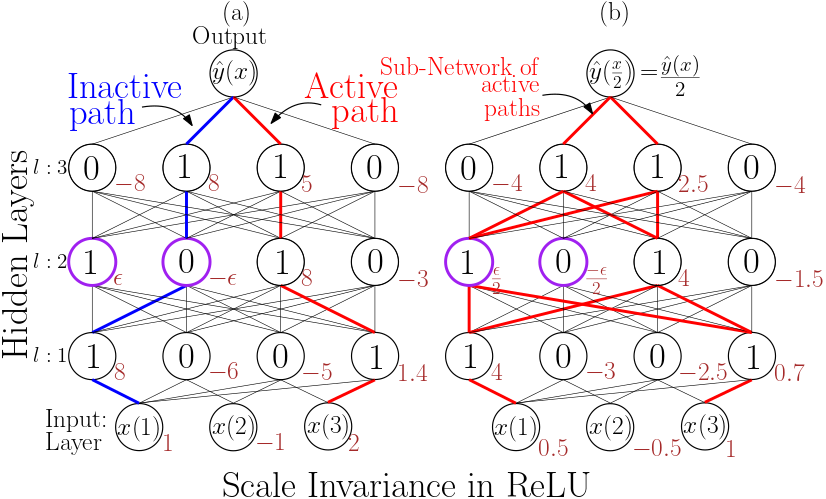
\includegraphics[scale=0.5]{figs/nn-subnet.png}
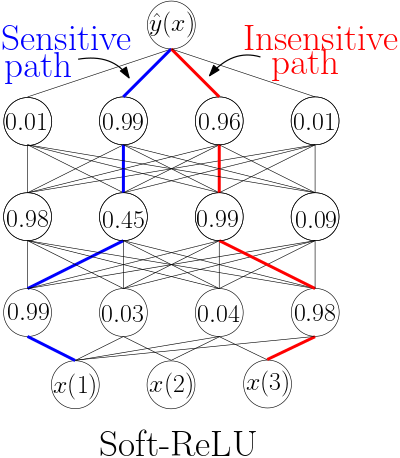
\includegraphics[scale=0.5]{figs/nnsoft.png}
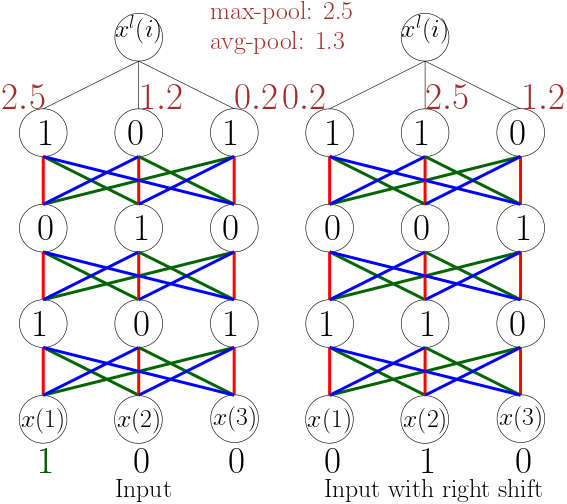
\includegraphics[scale=0.5]{figs/nnconv.png}
%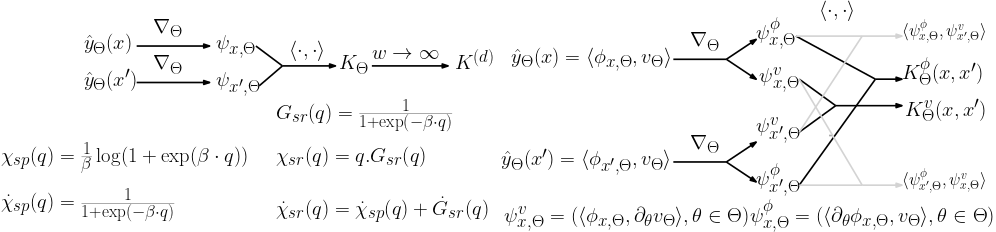
\includegraphics[scale=0.5]{figs/gradflow.png}
%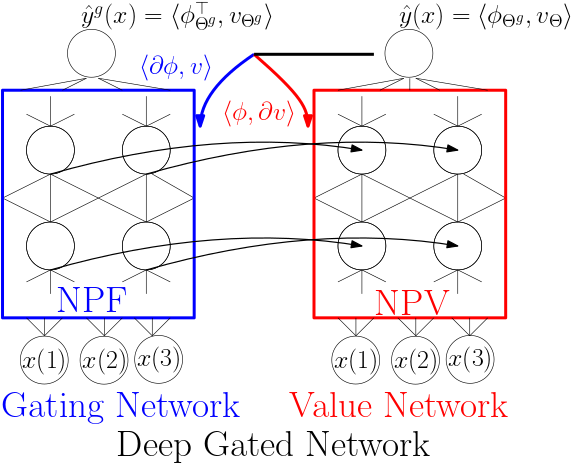
\includegraphics[scale=0.5]{figs/nntwin-blck.png}
%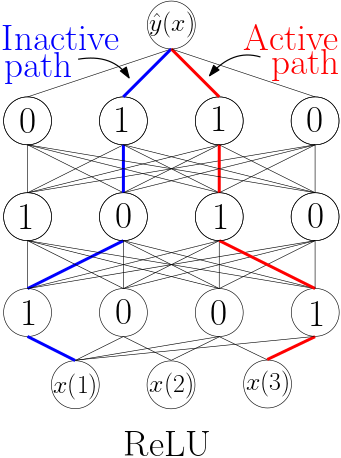
\includegraphics[scale=0.5]{figs/nn.png}
%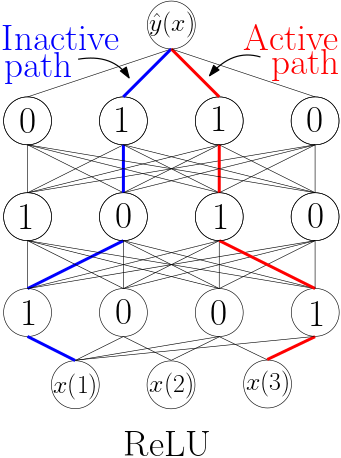
\includegraphics[scale=0.5]{figs/nn.png}
\end{tabular}
}
%\end{minipage}
%\begin{minipage}{0.18\columnwidth}
%\resizebox{\columnwidth}{!}{
%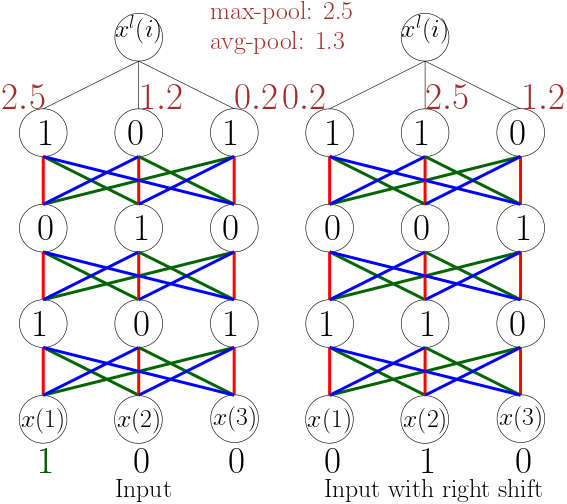
\includegraphics[scale=0.5]{figs/nnconv.png}
%}
%\end{minipage}
\caption{Cartoon illustration of usefulness of path-view and DGN framework.}
\label{fig:cartoon}
\end{figure*}
The \textbf{neural path feature} (NPF) of an input $x\in\R^{d_{in}}$ is given by 
\begin{align}\label{eq:npfdef}
\phi_{x,\Theta}\stackrel{def}=(x_s(\I_0(p))A_{\Theta}(x_s,p) ,p\in[P])\in\R^P,
\end{align}
where, for a path $p$, $\I_0(p)$ is the input node at which the path starts, and $A_{\Theta}(x_s,p)$ is its activity. \\
%By arranging the NPF of the $n$ input examples in a matrix $\Phi_t=(\phi_{x_s,\G_t},s\in[n])\in\R^{P\times n}$, we can express 
The \textbf{neural path value} (NPV) if given by  
\begin{align}\label{eq:npvdef}
v_{\Theta}\stackrel{def}=(\Pi_{l=1}^d \Theta(l,\I_{l-1}(p),\I_l(p)),p\in[P])\in\R^P
\end{align}
The zeroth and first-order terms of a DNN can be written as:
\begin{align}
\label{eq:zero}\text{(Zeroth-Order)}\quad: \quad \hat{y}_{\Theta}(x)&=\ip{\phi_{x,\Theta},v_{\Theta}}=\sum_{p\in [P]}x(\I(p))A_{\Theta}(x,p)v_{\Theta}(p)\\
\label{eq:first}\text{(First-Order)}\quad: \quad \partial \hat{y}_{\Theta}(x)&=\underbrace{\ip{\phi_{x,\Theta},\partial v_t}}_{\text{value gradient}}+ \underbrace{\ip{\partial\phi_{x,\Theta},v_{\Theta}}}_{\text{feature gradient}}\\&=\sum_{p\in [P]}x(\I(p)) A_{\Theta}(x,p) \partial(v_{\Theta}(p))+\sum_{p\in [P]}x(\I(p)) \partial(A_{\Theta}(x,p)) v_{\Theta}(p)\nn
\end{align}
\subsection{Information Flow via Sub-Networks}
$1.$ \textbf{Representational Power Vs Scale Invariance:} The ability of DNNs to fit data has been demonstrated in the past. \cite{ben} showed that DNNs can fit even random labels, and random pixels of standard datasets such as MNIST. However, we note that, for DNNs with ReLU, with no bias parameters, a dataset with $n=2$ points namely $(x,1)$ and $(x/2,-1)$ for some $x\in \R^{d_{in}}$ cannot be memorised. The reason is that the gating values are the same for both $x$ and $x/2$ (for that matter any positive scaling of $x$), and hence $\phi_{x/2,\Theta}= \phi_{x,\Theta}/2$, and thus it not possible to fit arbitrary values for $\hat{y}_t(x/2)$ and $\hat{y}_t(x)$, since $\hat{y}_t(x/2)= \hat{y}_t(x)/2$. Cartoons $(a)$ and $(b)$ in \Cref{fig:cartoon} illustrate this scale invariance for inputs $x=(1,-1,2)\in\R^3$ and $x/2=(0.5,-0.5,1)\in\R^3$:  when compared to $(a)$, pre-activation values and output of $(b)$ are scaled down by a factor $2$, and the gating values of $(a)$ and $(b)$ are identical.\\
$2.$ \textbf{Translation Invariance:} Consider a convolution network using $l$ layers of circular convolutions\footnote{Here, instead of zero-padding in the corners, we follow the convention that index $d_{in}+k$ will be interpreted as $k$, for $k>0$, and $-k$ will be interpreted as $d_{in}-k$.} with filter size $k'<d_{in}$ and unit stride, and let $x^l(i)$ be the output of the $i^{th}$ channel after either $\max$-/global-average-pooling. Looking at the third and fourth (from left) illustrations in \Cref{fig:cartoon}, it is easy to check the translation invariance property: each of the red, blue, green lines have the same path values due to weight sharing in the convolutional layers, this leads to a circular symmetry in the path values, due to which, a translation in the input will cause all the internal variable to translate, and final invariance results from the invariance of the $\max$/average operation.\\
$3.$ \textbf{Active Sub-Network:} For each input example, a set of gates are \emph{on} in each layer, and this gives rise to the sub-network of active paths for that input. This active sub-network can be said to hold the memory for a given input (see cartoon $(b)$ in \Cref{fig:cartoon}).

%\subsection{Information Flow: First-Order}

\textbf{First-Order Information Flow}\\
$1.$ \textbf{Value Gradient} $\ip{\phi_{x,\Theta},\partial v_\Theta}$ (see \eqref{eq:zero}) flows through the active sub-network. To see this, $\ip{\phi_{x,\Theta},\partial v_{\Theta}}=\sum_{p\in[P]}x(\I_0(p))A_{\Theta}(x,p)\partial v$, i.e., only paths $p$ with $A_{\Theta}(x,p)=1$ contribute to the summation and $\partial v_{\Theta}(p)$ is non-zero only for those weights through which the path $p$ passes.\\
$2.$ \textbf{Feature Gradient}  $\ip{\partial\phi_{x,\Theta},v_{\Theta}}=\sum_{p\in [P]}x(\I(p)) \partial(A_{\Theta}(x,p)) v_{\Theta}(p)$. Note that, in the case of ReLU activations the gating values are either $0$ or $1$, and hence $\partial(A_{\Theta}(x,p))=0$. However, the gating values and hence the path activities $A_{\Theta_t}(\cdot,\cdot)$ changes during training. This artefact arising due to non-differentiability can be fixed by considering a \emph{soft-ReLU} activation. 
%where, for a pre-activation input $q\in\R$ the output is given by $q\frac{1}{1+\exp(-\beta q)}$ as opposed to $q\mathbbm{1}_{\{q>0\}}$ of the ReLU. 
Soft-ReLU `trick' enables us to capture the terms related to feature learning in our analysis. The difference between hard and soft gates can be seen cartoons $(a)/(b)$ and $(c)$ in \Cref{fig:cartoon}, where negative/positive values lead to $0/1$ in the case of hard gating, and close to $0/1$ in the case of soft-gating.\\
$3.$ \textbf{Sensitive Sub-Network:} In a DNN with soft-ReLU, $\partial A_{\Theta}(x,p)=\sum_{l=1}^d \partial G_{x,\Theta}(l)\Pi_{l'\neq l}G_{x,\Theta}(l')$ is significant for those paths $p$ for which one of the $d-1$ gating values is close to $0.5$ (say such a gate is in layer $l$, and for such a gate $\partial G_{x,\Theta}$ is significant) and rest of the $d-2$ gates are close to $1$, so that $\Pi_{l'\neq l}G_{x,\Theta}(l')$ is significant. The set of paths for which $\partial A_{\Theta}(x,p)$ is significant, form the sensitive sub-network for that input. The sensitive paths are shown in cartoon $(c)$ of \Cref{fig:cartoon}. In the case of, standard ReLU, sensitive paths are those which contain one of the gates with pre-activation close to $0$, and rest of the $d-2$ gates are $1$.
\begin{comment}
\subsection{Deep Gated Network (DGN)}
The NPFs are zeroth-order features stored solely in the gates of a DNN. In this paper, we separate out the NPFs from the NPVs. To this end, we introduce the deep gated network (DGN) framework, wherein, the output of a hidden unit is obtained as a product of its pre-activation and a gating value. A DGN has two network namely i) the gating network which holds the gating values and hence the NPF, and ii) a value network which holds the NPVs. %We denote a DNG by $\N(\Theta_t;\G(\Tg_t,\beta)$ or simply $\N(\Theta_t;\Tg_t,\beta)$
\begin{table}[h]
\begin{minipage}{0.5\columnwidth}
\resizebox{\columnwidth}{!}{
\begin{tabular}{|c|c|}\hline
Gating Network: $\G(\Tg_t,\beta)$\\\hline
$z_{x,\Tg_t}(0)=x$  \\\hline
$q_{x,\Tg_t}(l)={\Tg_t(l)}^\top z_{x,\Tg_t}(l-1)$ \\\hline
$z_{x,\Tg_t}(l)=q_{x,\Tg_t}(l)\odot G_{x,\Tg_t}(l)$ \\\hline
{$\begin{aligned}\beta >0: G_{x,\Tg_t}(l,i)&=\frac{1+\epsilon}{1+\exp(-\beta q_{x,\Tg_t}(l,i))} \\ \beta=\infty: G_{x,\Tg_t}(l,i)&=\mathbbm{1}_{\{q_{x,\Tg_t}(l,i)>0\}}\end{aligned}$}\\\hline 
\end{tabular}
}
\end{minipage}
\begin{minipage}{0.5\columnwidth}
\resizebox{\columnwidth}{!}{
\begin{tabular}{|l|l|}\hline
\multicolumn{2}{|c|}{Value Network: $\N(\Theta_t;\G_t)$}\\\hline 
Input layer & $z_{x,\Theta_t}(0)=x$ \\\hline
Pre-activation & $q_{x,\Theta_t}(l)={\Theta_t(l)}^\top z_{x,\Theta_t}(l-1)$\\\hline
Layer output & $z_{x,\Theta_t}(l)=q_{x,\Theta_t}(l)\odot G_{x,t}(l)$ \\\hline
Final output & $\hat{y}_t(x)={\Theta_t(d)}^\top z_{x,\Theta_t}(d-1)$\\\hline
Gating Values& $\begin{aligned}\G_t\stackrel{def}=\{G_{x_{s},t}(l,i), \forall s\in[n],\\l\in[d-1],i\in[w]\}\end{aligned}$\\\hline
\end{tabular}
}
\end{minipage}
\caption{$q(l),z(l)$ and $G(l)$ are $w$-dimensional quantities}
\label{tb:dgn}
\end{table}
\end{comment}
%\section{Feature Learning}
\textbf{Sensitive Sub-Network:} For an input $x\in\R^{d_{in}}$, let $\P^{\S}_{x,t}(\tau_{\S})=\{p\in[P]: |\partial_{\tg} A_t(x,p)|\tau_{\S}\}$ be the set of paths, which have activations whose gradient to any of $\Tg\inrdnet$ is greater than some threshold $\tau>0$. Using the property that the slope of the sigmoid diminishes in the extremities, we note that for appropriate choices of $\tau_{\A}$ (sufficiently close to $1$) and $\tau_{\S}$ (large enough), $\P^{\S}(\tau_{S})\cup \P^{\A}(\tau_{\A})$.
We now take a re-look at the NTF and NTK matrices, and explicitly write down the terms related to feature learning. \hfill\\
$2.$ Let us take the case of classification with cross-entropy loss. Say we have trained till some $T$ epochs with good classification (say close to $100\%$) accuracy. Considering the fact that $\hat{y}_T=\Phi_{\Tg_T}v_{\Theta_T}$, the gradient with respect to $\Tg$ will change the NPF matrix $\Phi_{\Tg_T}$ in such a manner to reduce the loss, i.e., increase the margin of each of the classified examples. We test this hypothesis  of \emph{margin-increase} due to feature learning in the following toy experiment.\hfill\\
\textbf{A Toy Experiment:} We look at a simple neural network with $d_{in}=2$, $w=2$ and $1$-hidden layer (see first diagram on the left in \Cref{fig:feat}). The first layer weights is an identity matrix, and for input $x\in\R^2$ to the network, the first layer output is given by $z_{t}(i)=x(i)G_t(i),i=1,2$, where $G_t(i)=\frac{1}{1+\exp(-\tg(i))},i=1,2$. In this network, there are $2$ paths, and the NPF is given by $\phi_{x,t}=(x(1)G_t(1),x(2)G_t(2))\in \R^2$ (note that this mimics the general structure of the NPF as presented in \Cref{sec:expressivity}).
We check the performance of frozen-gates versus adaptable gates in this network. The dataset is $(x_s,y_s)_{s=1}^{n},n=1000$, wherein, for $s=,1,\ldots,500$, $x_s(1)\stackrel{iid}\sim U[0.1,1]$, and $x_s(2)\stackrel{iid}\sim U[-100,100]$, and $y_s=1$, and for $s=501,\ldots,1000$, $x_s(1)\stackrel{iid}\sim U[-0.1,-1]$, and $x_s(2)\stackrel{iid}\sim U[-100,100]$, and $y_s=-1$. We use the loss function $L_t=\frac{1}{n}\sum_{s=1}^n\frac{1}{1+exp(-y_s\hat{y}_t(x_s))}$. The maximum margin classifier in this case is: predict $+1$ if $x(1)>0$ and else predict $-1$. We trained the simple neural network using gradient descent with step-size of $0.1$, and initialisation $\Tg_0=\Theta_0=(0,0)\in\R^2$ for the following two cases: i) frozen-gates, wherein, we set $\Tg_0=\Tg_t=\Tg_0,\forall t\geq 0$, so that the input features are not transformed, and train only $\Theta_t$ ii) adaptable gates, wherein, we train both $\Tg_t$ and $\Theta_t$. While both cases train for $T=10^4$ epochs, for $T=10^3$ epochs only the model with adaptable gates trains successfully. The results are shown in \Cref{fig:feat}, notice that the right most plot shows that in the case when the gates are adapting, they learn to suppress the second co-ordinate (the scale of $\phi_{x_s,T}$ is from $-15$ to $15$ as opposed to $-100$ to $100$ in $x_s$).
\FloatBarrier
\begin{figure}[h]
\begin{minipage}{0.15\columnwidth}
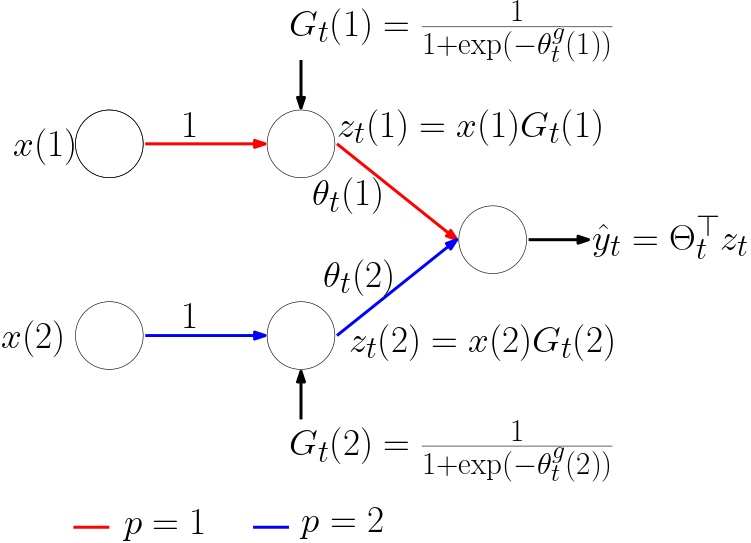
\includegraphics[scale=0.15]{figs/featlearn.png}
\end{minipage}
\hspace{50pt}
\begin{minipage}{0.8\columnwidth}
\resizebox{1\columnwidth}{!}{
\begin{tabular}{cccc}
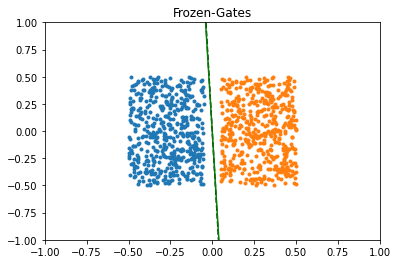
\includegraphics[scale=0.2]{figs/simple-1e2.png}
&
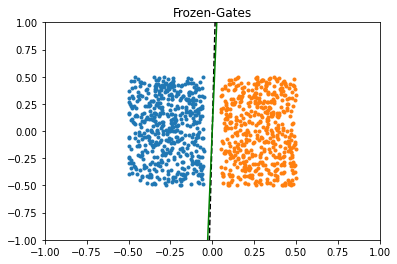
\includegraphics[scale=0.2]{figs/simple-1e3.png}
&
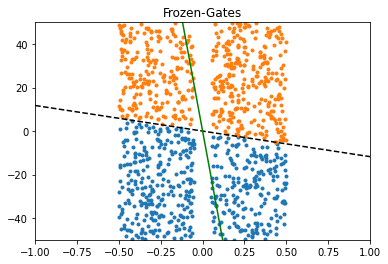
\includegraphics[scale=0.2]{figs/simple.png}
&
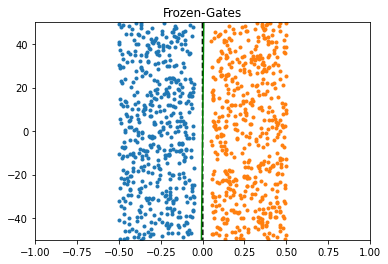
\includegraphics[scale=0.2]{figs/simple-1e4.png}
\\
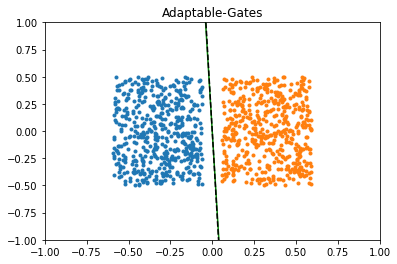
\includegraphics[scale=0.2]{figs/adapt-1e2.png}
&
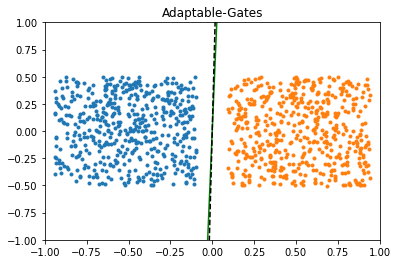
\includegraphics[scale=0.2]{figs/adapt-1e3.png}
&
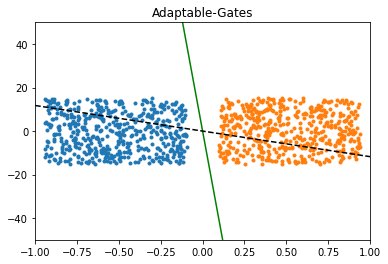
\includegraphics[scale=0.2]{figs/adapt.png}
&
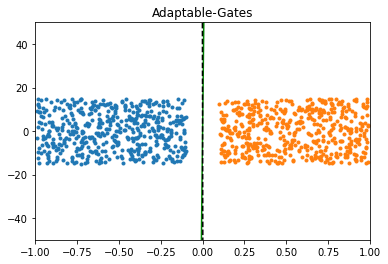
\includegraphics[scale=0.2]{figs/adapt-1e4.png}
\end{tabular}
}
\end{minipage}

\caption{From left: second and third plots shows the training performance of frozen and adaptable gates respectively. In both plots, the bold line in green is the classifier learnt in the case of adaptable gates, and the dotted black line is the classifier learnt in the case of frozen gates. Notice the transformation of the feature space in the case of adaptable gates.}
\label{fig:feat}
\end{figure}
$3.$ \textbf{An open question:} Informally speaking, in the above example, even though the gating parameters had $2$-degrees of freedom, it was nonetheless sufficient to adapt the features. Thus, perhaps we can hypothesise that subject to the `well-conditioned' ness of $K^a_t$, such margin increase can be perhaps achieved for all the $n$ examples.  However, in practice, both $\Tg_t$ as well as $\Theta_t$ change, and an open question is to understand how the joint optimisation and feature learning happens. 

\begin{comment}
\subsection{Kernels}\label{sec:kernels}
\subsubsection{Neural Path Kernel}
The NPF matrix is given by $\Phi_{\Theta}=(\phi_{x_s,\Theta},s\in[n])\in\R^{P\times n}$. The NPK matrix is then given by $H_{\Theta}=\Phi^\top_{\Theta}\Phi_{\Theta}$. The NPK matrix has a special structure as given in \Cref{lm:npk} below.
\begin{lemma}\label{lm:npk}
Let $p\rsa i$ denote the fact that path $p$ passes through input node $i\in[d_{in}]$, and let $\Lambda_{\Theta}(s,s')\stackrel{def}{=}\sum_{p\rsa i} A_{\Theta}(x_s,p) A_{\Theta}(x_{s'},p)$, $\forall s,s'\in[n]$, any $i\in [d_{in}]$. It follows that $H_{\Theta}= \Sigma\odot\Lambda_{\Theta}$, where $\odot$ stands for the Hadamard product, and $\Sigma \in \R^{n\times n}$ is the input Gram matrix.
\end{lemma}
In the \Cref{lm:npk} above, $\Lambda_{\Theta}\in\R^{n\times n}$ is the correlation matrix of the active sub-networks of different input pairs $s,s'\in[n]$. Note that the definition of $\Lambda$ is not dependent on the choice of input node $i$, because, the terms inside the summation depend only on the path followed from the first layer onwards and excludes the input node.\\
\subsubsection{Neural Tangent Kernel}
Using the `path-view', we obtain a different decomposition for the NTK matrix $K{\Theta}$, and compare our expression to the previously obtained expression in \Cref{eq:ntkold}. To this end, let us by define $d_{net}\times n$ matrices $\Psi^v_t$, and $\Psi^{\phi}_t$, whose entries are given by $\Psi^v_t(\theta,s)=\ip{\phi_{x_s,\Theta},\partial_{\theta}v_{\Theta}}$, and  $\Psi^{\phi}_t(\theta,s)=\ip{\partial_{\theta}\phi_{x_s,\Theta}, v_{\Theta}}$. Now, we have the following NTK decomposition (for a soft-ReLU DNN):
\begin{align}\label{eq:ntknew}
K_{\Theta}=K^v_{\Theta}+K^{\phi}_{\Theta}+(\Psi^v_\Theta)^\top \Psi^{\phi}_{\Theta} +(\Psi^{\phi}_\Theta)^\top \Psi^{v}_{\Theta},\,\text{where},
\end{align}
$K^v_{\Theta}$ is the NTK of path values due to the value gradient, $K^{\phi}_{\Theta}$ is the NTK of the features due to the feature gradient, and $(\Psi^v_\Theta)^\top \Psi^{\phi}_{\Theta} +(\Psi^{\phi}_\Theta)^\top \Psi^{v}_{\Theta}$, is a symmetric matrix which is the cross-term obtained as an interaction of the value and the feature gradients. %We now list the salient points about the decomposition in \eqref{eq:ntknew}. The recursive relationship in \eqref{eq:ntkold} is due to the fact that both zeroth-order (forward propagation) and first-order (backward propagation) information use a layer after layer expression for information flow. Also, \eqref{eq:ntkold} derives a limiting matrix ($w\ra\infty$) that occurs at a random $\Theta_0$. On the contrary, \eqref{eq:ntknew} holds for any parameter setting and for finite $w$ and $d$.\\
%\subsection{Neural Path Kernel and Optimisation}
%\subsection{Gate Dynamics and Feature Learning}
%$\bullet$ $(\Psi^v_\Theta)^\top \Psi^{\phi}_{\Theta} +(\Psi^{\phi}_\Theta)^\top \Psi^{v}_{\Theta}$, is a symmetric matrix which is the cross-term obtained as an interaction of the value and the feature gradients.
\section{Neural Tangent Kernel in Prior Works}
The NTK matrix has also been used to design pure-kernel based methods \cite{arora2019exact} and provide generalisation bounds \cite{cao2019generalization}.\\
\textbf{NTK in prior works:} Before we connect the NPK and the NTK using the `path-view', we will first look at prior works based on NTK. Prior works have used the following recursive definition or its variants, wherein, for layers $l=1,\ldots, d-1$, we define matrices:
\begin{align}\label{eq:ntkold}
&\tilde{K}^{(1)}(s,s')=\Sigma^{(1)}(s,s')=\Sigma(s,s'), M^{(l)}_{ss'}=\left[\begin{matrix}\Sigma^{(l)}(s,s) & \Sigma^{(l)}(s,s')\\ \Sigma^{(l)}(s',s) & \Sigma^{(l)}(s',s')\end{matrix}\right]\in \R^2,\\
&\Sigma^{(l+1)}(s,s')= 2\cdot\mathbb{E}_{(q,q')\sim N(0,M_{ss'}^{(l)})} \left[\chi(q)\chi(q')\right], \dot{\Sigma}^{(l+1)}(s,s')= 2\cdot\mathbb{E}_{(q,q')\sim N(0,M_{ss'}^{(l)})}\left[\dot{\chi}(q)\dot{\chi}(q')\right],\nn\\
&\tilde{K}^{(l+1)}=\tilde{K}^{(l)}\odot \dot{\Sigma}^{(l+1)}+\Sigma^{(l+1)},\nn
\end{align}
where $s,s'\in[n]$ are two input examples in the dataset, $\Sigma$ is the data Gram matrix, $\dot{\chi}$ stands for the derivative of the activation function with respect to the pre-activation input, $N(0,M)$ stands for the mean-zero Gaussian distribution with co-variance matrix $M$. The final limiting matrix is given by $K^{(d)}=\left(\tilde{K}^{(d)}+\Sigma^{(d)}\right)/2$. Prior works show that at randomised initialisation $\Theta_0$, $K_{\Theta_0}\ra K^{(d)}$ as $w\ra \infty$.
$K^{\phi}_{\Theta}$ is the NTK of the features, and describes the dynamics of feature learning due to the flow of the feature gradients, which, for each input example, decides which of the sensitive yet inactive paths should become active, and which of the sensitive yet active paths should become inactive. The NTK of features can be expanded as $K^{\phi}_{\Theta}=\sum_{\theta \in \Theta}\partial_{\theta} \Phi^\top_{\theta}v_{\Theta}v^\top_{\Theta}\partial_{\theta}\Phi_{\Theta}$. The significance here is that $\partial \Phi_{\Theta}$ terms contain, $\partial A_{\Theta}(\cdot,\cdot)$, which in turn contains $\partial G$ terms, which in turn contains $\dot{G}$ term which is the derivative of the gate with respect to its pre-activation input. NTK expression in prior works \eqref{eq:ntkold} only capture the $\chi$ and $\dot{\chi}$ terms. As shown in \Cref{fig:actgate}, only $\dot{G}$ (right-most plot) captures the gates that are in the verge of transition (either from $0$ to $1$ or from $1$ to $0$).
%$\bullet$ $(\Psi^v_\Theta)^\top \Psi^{\phi}_{\Theta} +(\Psi^{\phi}_\Theta)^\top \Psi^{v}_{\Theta}$, is a symmetric matrix which is the cross-term obtained as an interaction of the value and the feature gradients.
\FloatBarrier
\begin{figure}[h]
%\begin{minipage}{0.78\columnwidth}
\resizebox{\columnwidth}{!}{
\begin{tabular}{ccc}
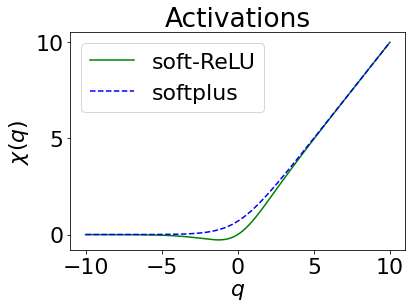
\includegraphics[scale=0.4]{figs/act.png}
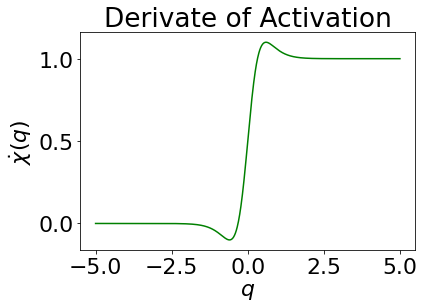
\includegraphics[scale=0.4]{figs/der-act.png}
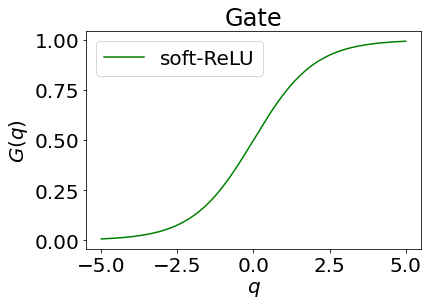
\includegraphics[scale=0.4]{figs/gate.png}
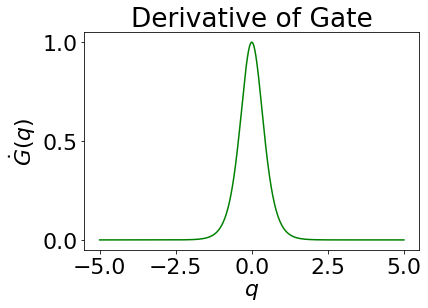
\includegraphics[scale=0.4]{figs/der-gate.png}
%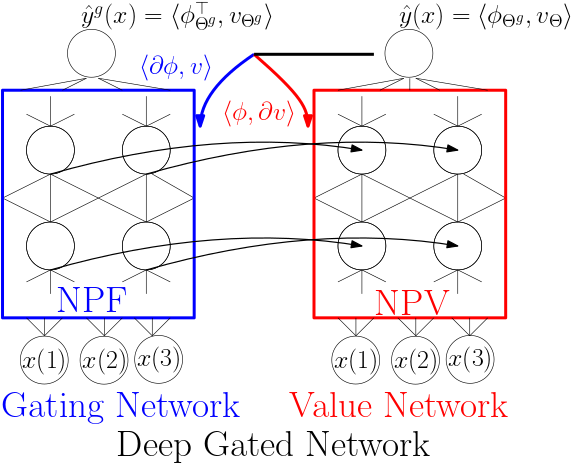
\includegraphics[scale=0.5]{figs/nntwin-blck.png}
%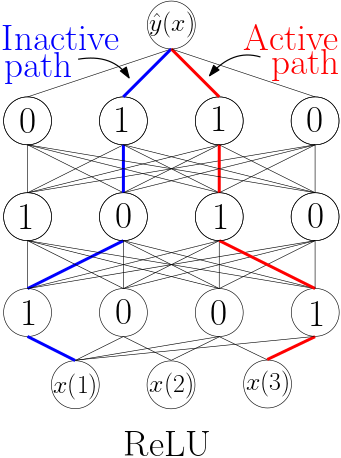
\includegraphics[scale=0.5]{figs/nn.png}
%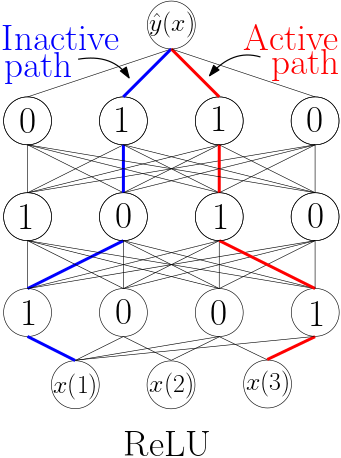
\includegraphics[scale=0.5]{figs/nn.png}
\end{tabular}
}
%\end{minipage}
%\begin{minipage}{0.18\columnwidth}
%\resizebox{\columnwidth}{!}{
%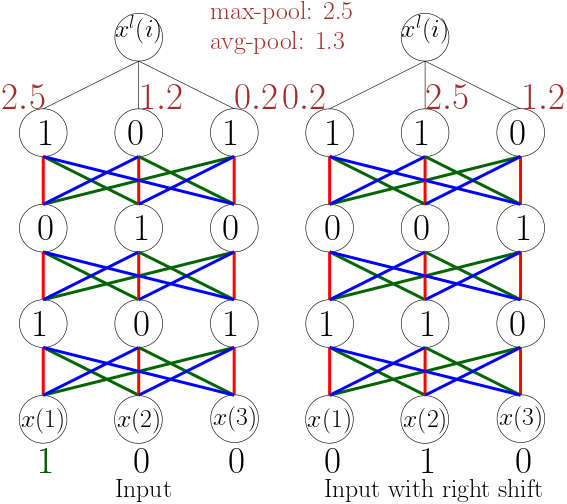
\includegraphics[scale=0.5]{figs/nnconv.png}
%}
%\end{minipage}
\caption{Activations and Gates}
\label{fig:actgate}
\end{figure}
\end{comment}